\documentclass[12pt]{article}
\usepackage{float}
\usepackage{graphicx}
\usepackage[font=small,labelfont=bf]{caption}
\usepackage{xcolor}
\usepackage{hyperref}

\pagestyle{empty}
\setcounter{tocdepth}{4}
\setcounter{secnumdepth}{4}

\topmargin=0cm
\oddsidemargin=0cm
\textheight=22.0cm
\textwidth=16cm
\parindent=0cm
\parskip=0.15cm
\topskip=0truecm
\raggedbottom
\abovedisplayskip=3mm
\belowdisplayskip=3mm
\abovedisplayshortskip=0mm
\belowdisplayshortskip=2mm
\normalbaselineskip=12pt
\normalbaselines

\begin{document}

\definecolor{light-gray}{gray}{0.95}
\newcommand{\code}[1]{\colorbox{light-gray}{\texttt{#1}}}

\vspace*{0.5in}
\centerline{\bf\Large Design Document - Iteration 2}

\vspace*{0.5in}
\centerline{\bf\Large Team PA-PI-a}

\vspace*{0.5in}
\centerline{\bf\Large 18 March 2018}

\vspace*{1.5in}
\begin{table}[htbp]
\caption{Team}
\begin{center}
\begin{tabular}{|r | c|}
\hline
Name & ID Number \\
\hline\hline
Melanie Taing & 40009850 \\
Laurie Gagnon & 22943433 \\
Wayne Yiel Leung & 26586988 \\
Jordan Rutty & 27300107 \\
Alice Barkhouse & 27486782 \\
Michael Foo & 40000225 \\
Pierre-Andre Leger & 40004010 \\
Colin Greczkowski & 40001600 \\
\hline
\end{tabular}
\end{center}
\end{table}

\clearpage

\tableofcontents
\clearpage

\listoffigures
\clearpage

\section{Introduction}
The purpose of this document is to describe and provide details for the design and
implementation of the second iteration of the MyMoney application.\\

The following pages will cover the rational of the architectural design, as well as the
subsystem interface specifications and details on their implementation. Finally, we will
describe three dynamic design scenarios based on use cases specified in the documentation
for iteration 1.

\section{Architectural Design} \label{sec:arch}
The MyMoney application is implemented using a model-view-controller (MVC) architecture. This section will cover the architectural diagram for the MVC as well as the subsystem interface specifications.
\newpage
\subsection{Architectural Diagram}

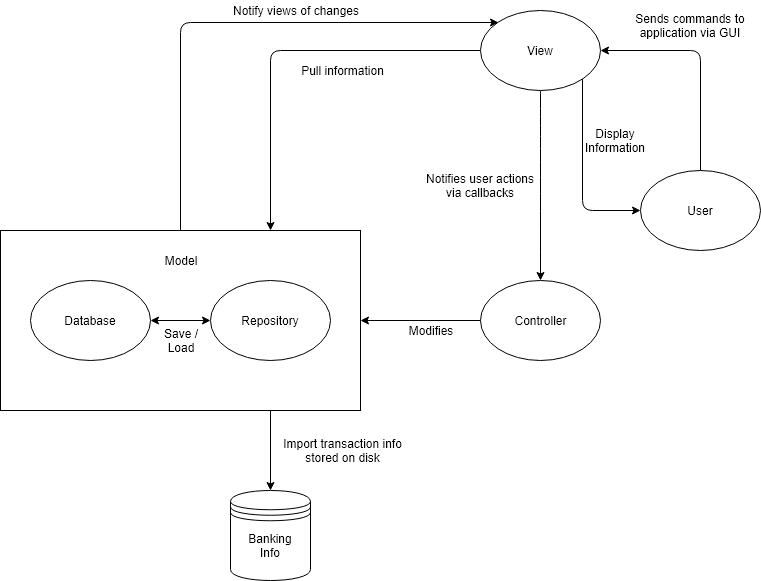
\includegraphics[width=\textwidth,height=\textheight,keepaspectratio]{diagrams/UML/MVC.png}
\captionof{figure}{High level structure of MVC architecture}\bigskip
The model contains all the information related to the transactions and the accounts that the user wishes to track. It consists of an SQL database used to serialize and deserialize   the information between user sessions and a repository with which the rest of the application interacts. Modifications to the repository are saved on-the-fly to the database while the program is running. The view displays the accounts and transactions loaded into the model (repository) and offers interactive elements that the user can interact with. In essence, it is a GUI. The controller handles user input from the view (GUI) and then acts on the model accordingly by adding, modifying or deleting transactions or accounts.\\

The main advantage of using an MVC pattern is the separation of concerns. As will be demonstrated in the next section, by enforcing each subsystem to depend strictly on \code{Interface} types when communicating with each other, we can reduce dependencies and greatly increase modularity.



\subsection{Subsystem Interface Specifications}

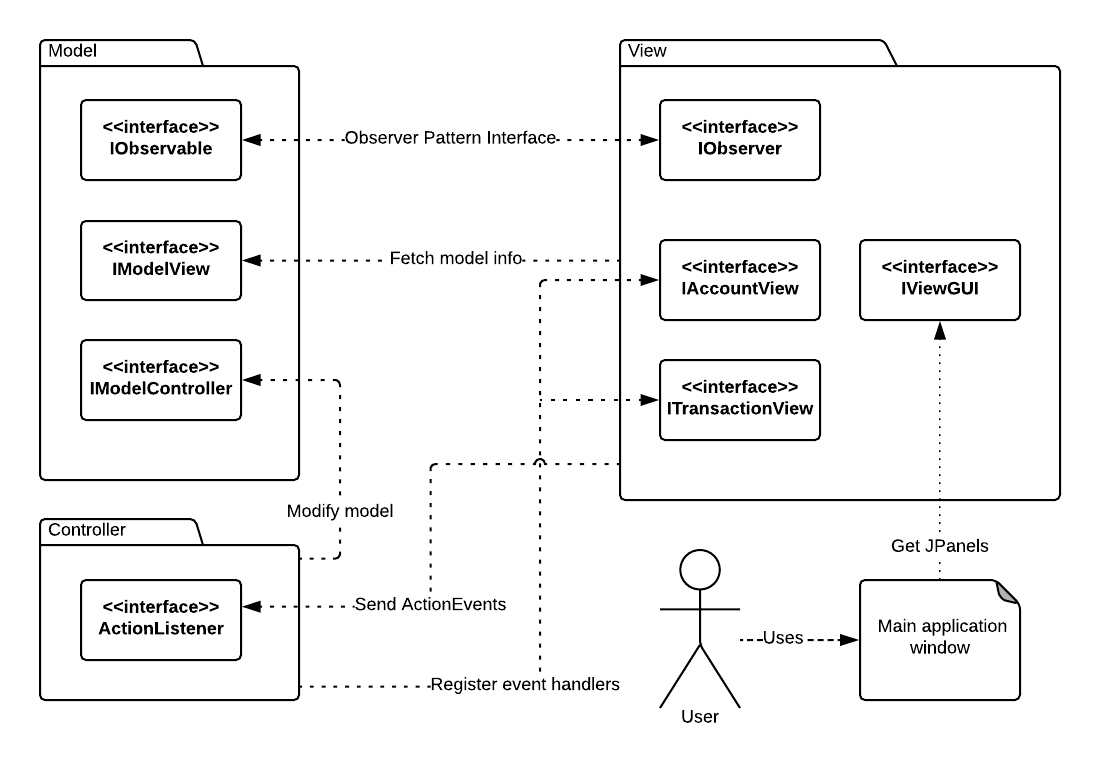
\includegraphics[width=\textwidth,height=\textheight,keepaspectratio]{diagrams/UML/Subsystem.png}
\captionof{figure}{Subsystem specification diagram}\bigskip

\subsubsection{Model - View : Observer Pattern}
The interfaces \code{IObservable} and \code{IObserver} form the observer pattern between the model and the view.\\

\code{IObserver}
\begin{itemize}
	\item \code{update()} : Called by an \code{IObservable} object. This should trigger internal logic in the observer to allow it to update its view on the model.
\end{itemize}\bigskip

\code{IObservable}
\begin{itemize}
	\item \code{attachObserver(IObserver)} : Attach an observer to this object.
	\item \code{detachObserver(IObserver)} : Detach an observer from this object.
	\item \code{notifyObservers()} : Call the \code{update()} method on all attached observers. Whenever the state of the model changes, it should call this function to allow its attached observers to update their views.
\end{itemize}\bigskip

\subsubsection{Model : IModelView Interface}
The \code{ImodelView} interface exposes methods to allow the view to fetch information from the the model.\\
\begin{itemize}
	\item \code{getTransactions(Integer accountId)} : Returns a list of \code{Transaction} objects belonging to the specified accountId. If there are no transactions for the account or the account does not exist, it will return an empty list.
	\item \code{getAllAccounts()} : Returns a list of all the \code{Account} objects for the current user.
\end{itemize}

\subsubsection{Model : IModelController Interface}
The \code{IModelController} interface exposes methods to allow the controller to modify the model.\\
\begin{itemize}
	\item \code{saveTransaction(Transaction)} : Saves the given \code{Transaction} object to the repository and updates the SQL database. If the ID of the transaction is 0, creates a new entry. Otherwise, updates the existing one.
	\item \code{saveAccount(Account)} : Saves the given \code{Account} object to the repository and updates the SQL database. If the ID of the account is 0, creates a new entry. Otherwise, updates the existing one.
	\item \code{deleteTransaction(Transaction)} : Deletes the specified transaction from both the repository and the SQL database.
	\item \code{deleteAccount(Account)} : Deletes the specified account from both the repository and the SQL database.
	\item \code{importTransactions(String path, Integer accountId)} : Constructs and saves \code{Transactions} objects to the repository and SQL databse from a .csv file located at the specified path. The format of the .csv file should be well defined.
\end{itemize}

\subsubsection{View : IAccountView}
The \code{IAccountView} interface exposes methods to allow the controller to register event listeners for user actions (buttons clicks) and have access to the content of the form fields filled by the user.\\
The callback system uses Java's \code{ActionEvent} class. 
\begin{itemize}
	\item \code{registerAddActionCallback(ActionListener, String)} : Attaches the specified listener to the GUI element that should trigger the "Add" action and set the event's action command to the specified string (should be "Add").
	\item \code{registerUpdateActionCallback(ActionListener, String)} : Attaches the specified listener to the GUI element that should trigger the "Update" action, and set the event's action command to the specified string (should be "Update").
	\item \code{registerDeleteActionCallback(ActionListener, String)} : Attaches the specified listener to the GUI element that should trigger the "Delete" action and set the event's action command to the specified string (should be "Delete").
	\item \code{getBankInput()} : Returns a string consisting of the content of the BankName field in the GUI.
	\item \code{getNicknameInput()} : Returns a string consisting of the content of the Nickname field in the GUI.
	\item \code{getBalanceInput()} : Returns an Integer consisting of the content of the Balance field in the GUI.
	\item \code{getSelectedAccountId()} : Returns a Integer consisting of the ID of the account currently selected by the user.
	\item \code{setSelection(Integer)} : Overrides the user's current account selection. This method mostly improves user experience (for example, automatically selects a new account when it is created).
\end{itemize}

\subsubsection{View : ITransactionView}
The \code{ITransactionView} interface exposes methods to allow the controller to register event listeners for user actions (buttons clicks) and have access to the content of the form fields filled by the user.\\
The callback system uses Java's \code{ActionEvent} class.
\begin{itemize}
	\item \code{registerAddActionCallback(ActionListener, String)} : Attaches the specified listener to the GUI element that should trigger the "Add" action and set the event's action command to the specified string (should be "Add").
	\item \code{registerUpdateActionCallback(ActionListener, String)} : Attaches the specified listener to the GUI element that should trigger the "Update" action and set the event's action command to the specified string (should be "Update").
	\item \code{registerDeleteActionCallback(ActionListener, String)} : Attaches the specified listener to the GUI element that should trigger the "Delete" action and set the event's action command to the specified string (should be "Delete").
		\item \code{registerImportActionCallback(ActionListener, String)} : Attaches the specified listener to the GUI element that should trigger the "Import" action and set the event's action command to the specified string (should be "Import").
	\item \code{getTypeInput()} : Returns a string consisting of the content of the Type field in the GUI.
	\item \code{getDateInput()} : Returns a string consisting of the content of the Date field in the GUI.
	\item \code{getDescriptionInput()} : Returns a string consisting of the content of the Description field in the GUI.
	\item \code{getAmountInput()} : Returns an Integer consisting of the content of the Amount field in the GUI.
	\item \code{getSelectedAccountId()} : Returns a Integer consisting of the ID of the account currently selected by the user.
	\item \code{getSelectedTransactionId()} : Returns a Integer consisting of the ID of the transaction currently selected by the user.
	\item \code{setSelection(Integer)} : Overrides the user's current transaction selection. This method mostly improves user experience (for example, resetting the current selection when a transaction is deleted)
\end{itemize}

\subsubsection{View : IViewGUI}
The \code{IViewGUI} interface exposes a single method that returns a \code{JPanel} object. It is only used by the main application window.
\begin{itemize}
	\item \code{getPanel()} : Returns the topmost parent \code{JPanel} of this view. It is meant to be used by the main application window to populate its frame.
\end{itemize}

\subsubsection{Controller : ActionListener}
The controller only needs to listen to events triggered by the user's input. From the other subsystems' perspective, it implements a single interface with a single method.
\begin{itemize}
	\item \code{actionPerformed(ActionEvent)} : Event handler for \code{ActionEvent} events created by the view. The controller registers its handlers by using the \code{IAccountView} or \code{ITransactionView} interfaces provided by the view(s).
\end{itemize}


\newpage
\section{Detailed Design} \label{sec:detail}

This section will cover the implementation details for each subsystem. Before moving on, a quick overview of the basic types used by the system is in order.\\
\\
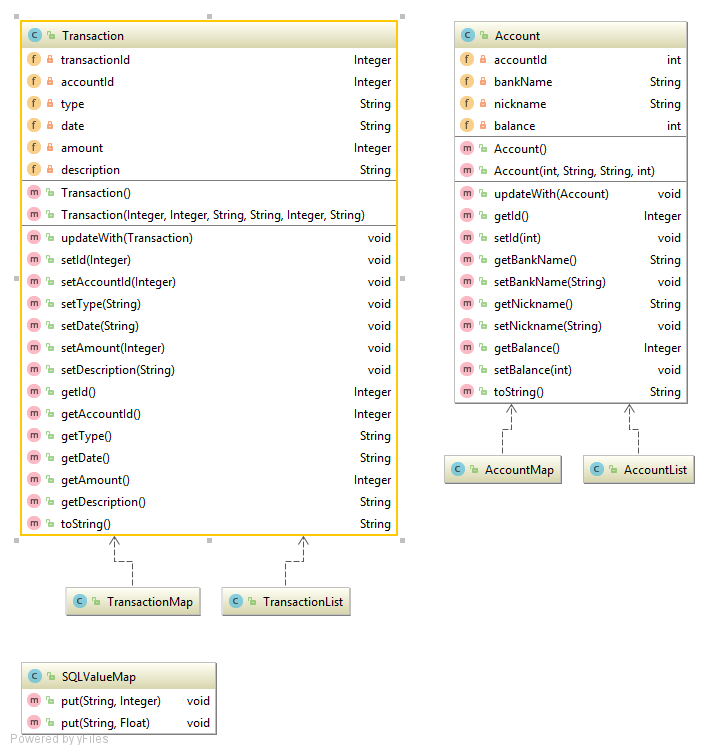
\includegraphics[width=\textwidth,height=\textheight,keepaspectratio]{Diagrams/UML/Types.png}
\captionof{figure}{Overview of basic types}\bigskip

\newpage
The \code{Transaction} and \code{Account} are nothing more than plain old data structures with public read and write access. They both inherit from the \code{AbstractUniqueId} class which holds the ID that will be used as primary key for the database. The \code{SQLValueMap} is a helper class  that derives from Java's \code{HashMap} and overrides the \code{put()} method to quickly convert the \code{value} of the (key,value) pair into a string. \code{SQLValueMaps} instances are extensively used when building strings that are sent to the SQL database.\\

In order to simplify the following class diagrams, dependencies on these types are to be assumed and have been omitted.\\

Links to javadoc generated documentation:\\
\href{run:javadoc/AbstractUniqueId.html}{AbstractUniqueId abstract class}\\
\href{run:javadoc/Account.html}{Account class}\\
\href{run:javadoc/Transaction.html}{Transaction class}\\
\href{run:javadoc/SQLValueMap.html}{SQLValueMap class}\\

\subsection{Model}

\subsubsection{Design Diagram}

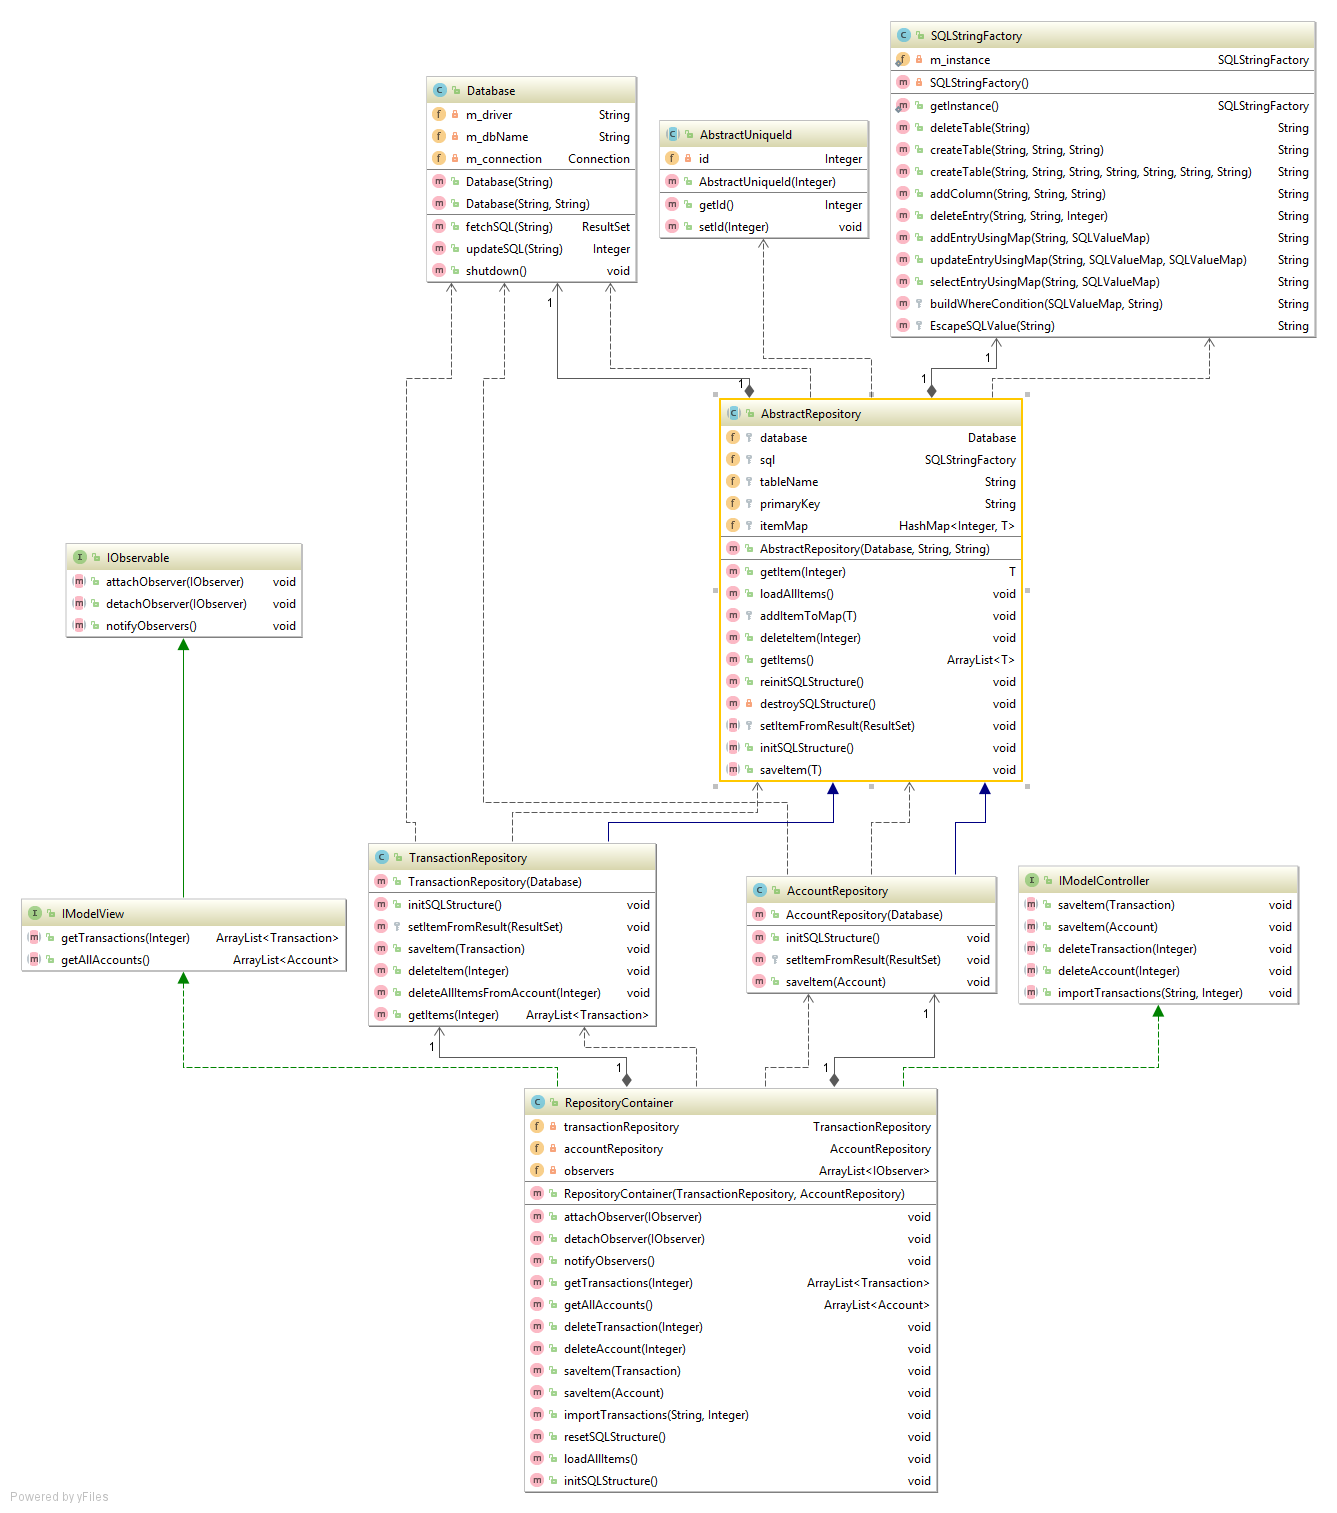
\includegraphics[width=\textwidth,height=\textheight,keepaspectratio]{Diagrams/UML/Model.png}
\captionof{figure}{Model subsystem class diagram}\bigskip

\newpage
The model subsystem consists of two main parts. The first is the \code{RepositoryContainer} that interfaces with the rest of the application. It owns the \code{TransactionRepository} and \code{AccountRepository} instances and passes read or write commands to each as they are received from the controllers. It also notifies the views of any CRUD operations using the observer pattern.\\

The second part consists of the SQL database. This is where all information is serialized to allow access between user sessions. It is continuously updated by the repositories as modifications are made. SQL queries to the database can easily be created by using the singleton \code{SQLStringFactory}.\\

\subsubsection{Units Description}

Links to javadoc generated documentation:\\
\href{run:javadoc/IObservable.html}{IObservable interface}\\
\href{run:javadoc/IModelView.html}{IModelView interface}\\
\href{run:javadoc/IModelController.html}{IModelController interface}\\
\\
\href{run:javadoc/AbstractRepository.html}{AbstractRepository abstract class}\\
\href{run:javadoc/AccountRepository.html}{AccountRepository class}\\
\href{run:javadoc/TransactionRepository.html}{TransactionRepository class}\\
\href{run:javadoc/RepositoryContainer.html}{RepositoryContainer class}\\
\\
\href{run:javadoc/Database.html}{Database class}\\
\href{run:javadoc/SQLStringFactory.html}{SQLStringFactory class}\\

\subsection{View}

\subsubsection{Design Diagram}

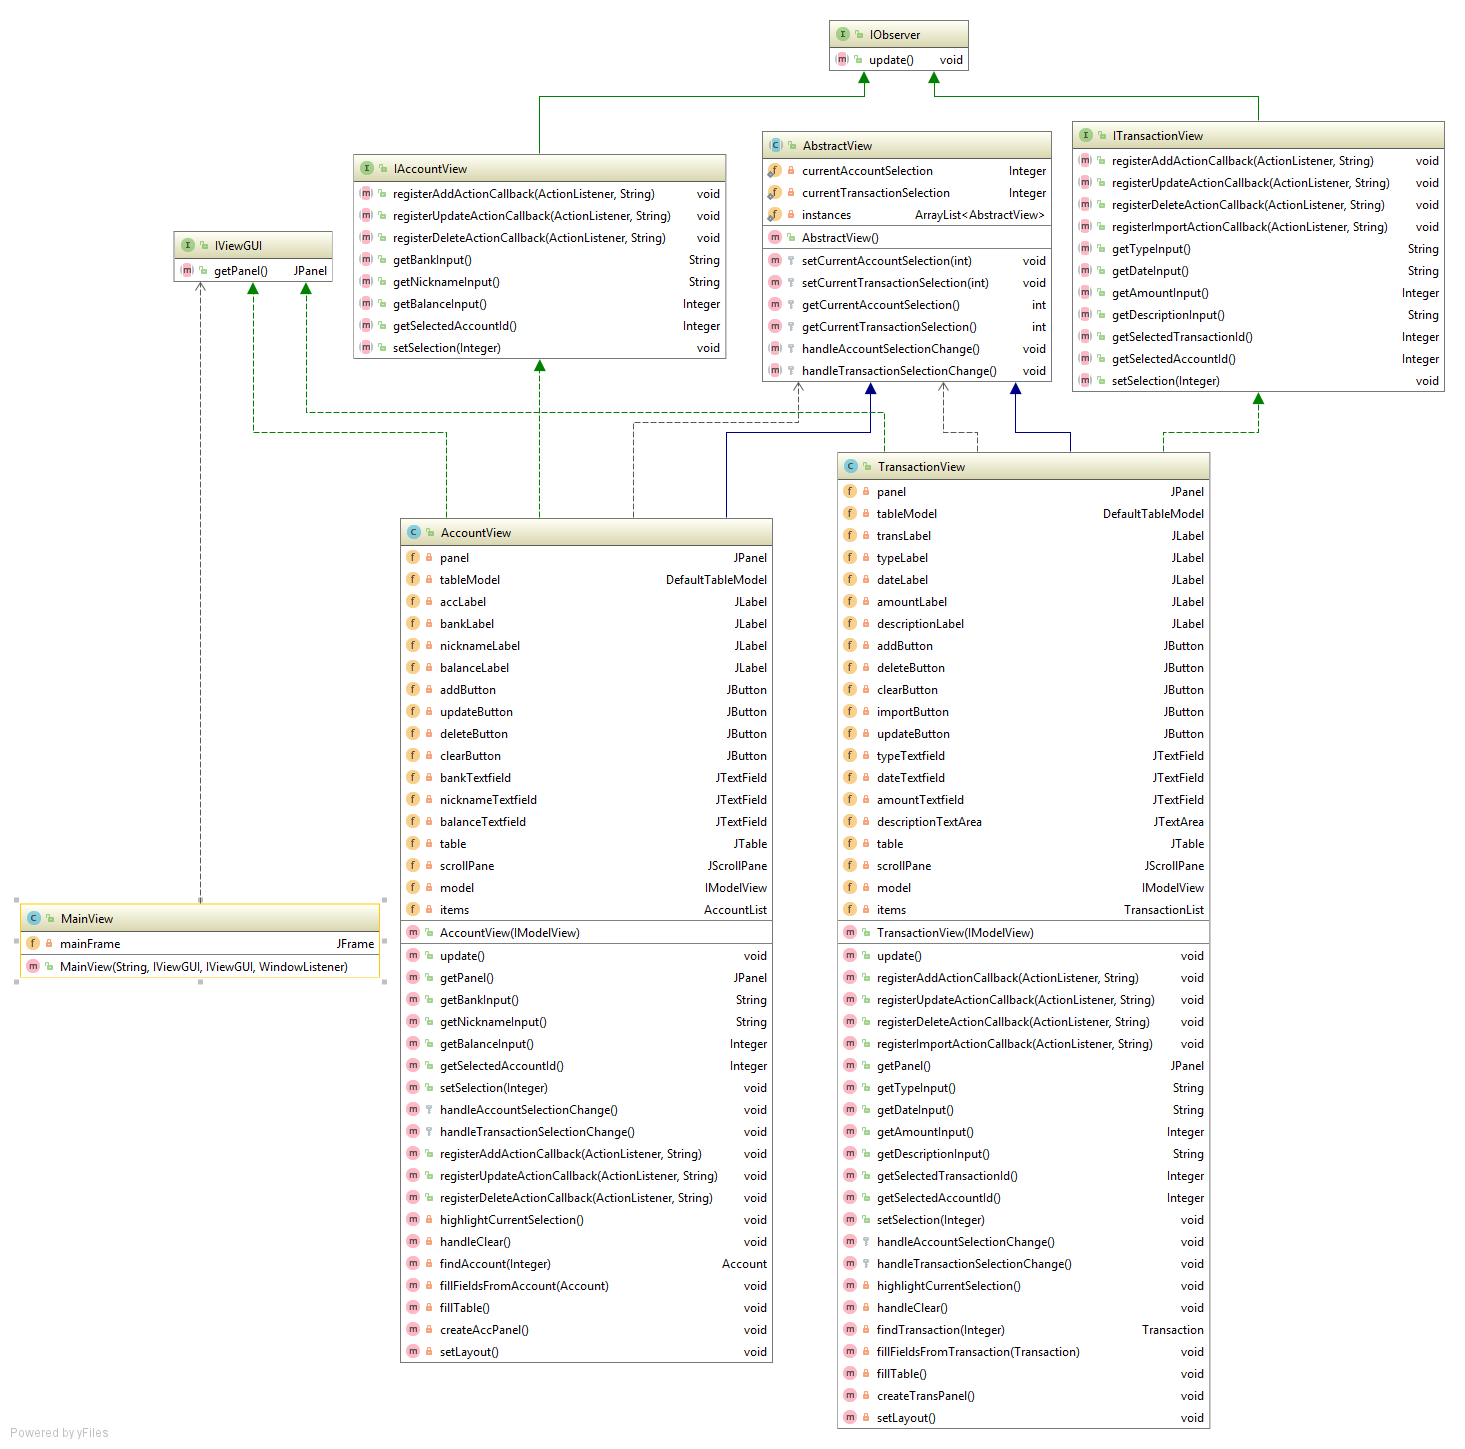
\includegraphics[width=\textwidth,height=\textheight,keepaspectratio]{Diagrams/UML/View.png}
\captionof{figure}{View subsystem class diagram}\bigskip

\newpage
The view subsystems consists of two concrete implementations, one for transactions and the other for accounts. They both implement the required interfaces for the other subsystems. Their roles are to update themselves when the model changes via their observer pattern implementation as well as sending events to the controller's registered callbacks methods whenever an action is required from the user input.\\

\subsection{Units Description}

Links to javadoc generated documentation:\\
\href{run:javadoc/IObserver.html}{IObserver interface}\\
\href{run:javadoc/IAccountView.html}{IAccountView interface}\\
\href{run:javadoc/IViewGUI.html}{IViewGUI interface}\\
\href{run:javadoc/ITransactionView.html}{ITransactionView interface}\\
\\
\href{run:javadoc/AbstractView.html}{AbstractView abstract class}\\
\href{run:javadoc/AccountView.html}{AccountView class}\\
\href{run:javadoc/TransactionView.html}{TransactionView class}\\

\subsection{Controller}

\subsubsection{Design Diagram}

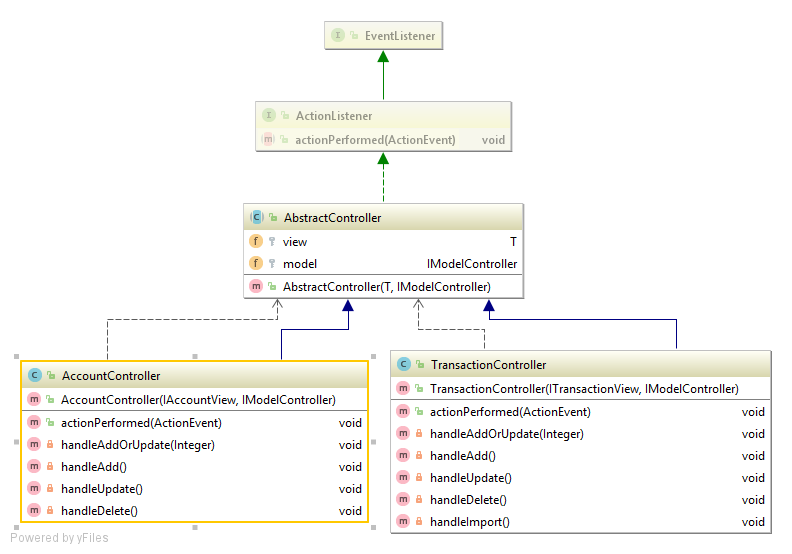
\includegraphics[width=\textwidth,height=\textheight,keepaspectratio]{Diagrams/UML/Controller.png}
\captionof{figure}{Controller subsystem class diagram}\bigskip

The controller subsystem is very slim. It consists only of two concrete implementations, one for accounts and the other for transactions. It registers event handlers to the views on creation and calls the appropriate methods on the model through the \code{IModelController} interface when action is required by the user.

\subsubsection{Units Description}

\href{run:javadoc/AbstractController.html}{AbstractController abstract class}\\
\href{run:javadoc/AccountController.html}{AccountController class}\\
\href{run:javadoc/TransactionController.html}{TransactionController class}\\

\newpage
\section{Dynamic Design Scenarios}
To illustrate the interactions between the difference classes of our system, we have drawn sequence diagrams for the main features of our program. For simplicity, the model interface is the lowest layer of abstraction in these diagrams. The final section illustrates the internal structure of the model to complement the higher level diagrams.

\subsection{Add an account} \label{sec:addAccount}
The first scenario illustrates the addition of an account to the system. The user completes the required text fields and presses the "Add" button, which sends an \code{ActionEvent} the \code{AccountController}. The controller then gathers and validates the inputs. If they are valid, the controller constructs an \code{Account} object and initializes it using the info gathered from the view. Finally, the object is saved by calling the model's \code{saveAccount()} method. See \ref{sec:modelSaveDetail} for the sequence diagram from the model's perspective once the call to \code{saveAccount()} is made. The sequence of calls for adding a \code{Transaction} is fundamentally the same.\\
\\
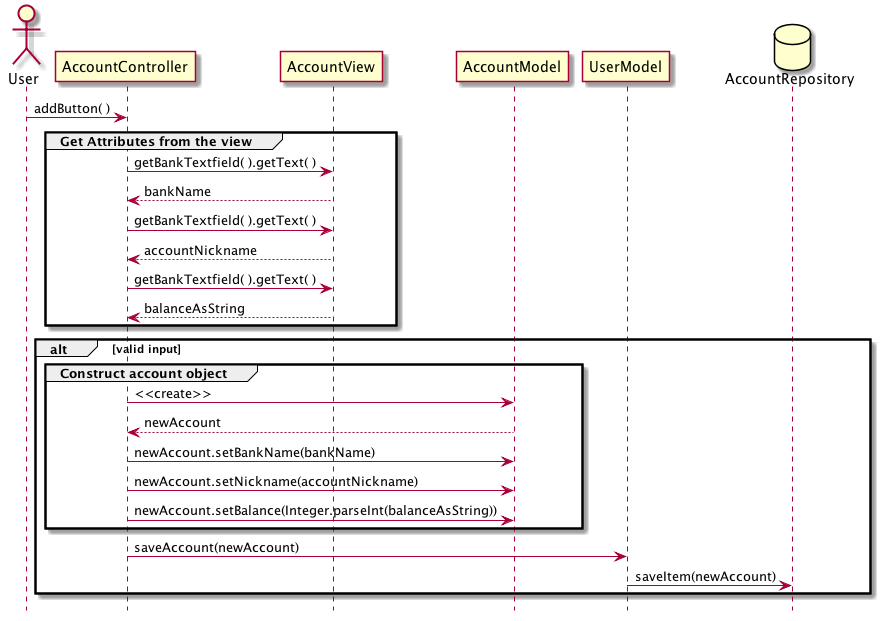
\includegraphics[width=\textwidth,height=\textheight,keepaspectratio]{diagrams/sequence/addAccount.png}
\captionof{figure}{Adding an account}
\bigskip

\subsection{Update an account}
Updating and existing \code{Account} is very similar to creating a new one. The one difference is that the user must first select an entry from the view. The fields will then update to show the selected \code{Account}'s information. The user can then modify the fields as desired and press the "Update" button when ready. The flow is then identical to \ref{sec:addAccount}, with the exception that the \code{AccountController} will set the created \code{Account} object's ID from the one selected by the user. Again, the sequence of calls for updating a \code{Transaction} is fundamentally the same.\\
\\
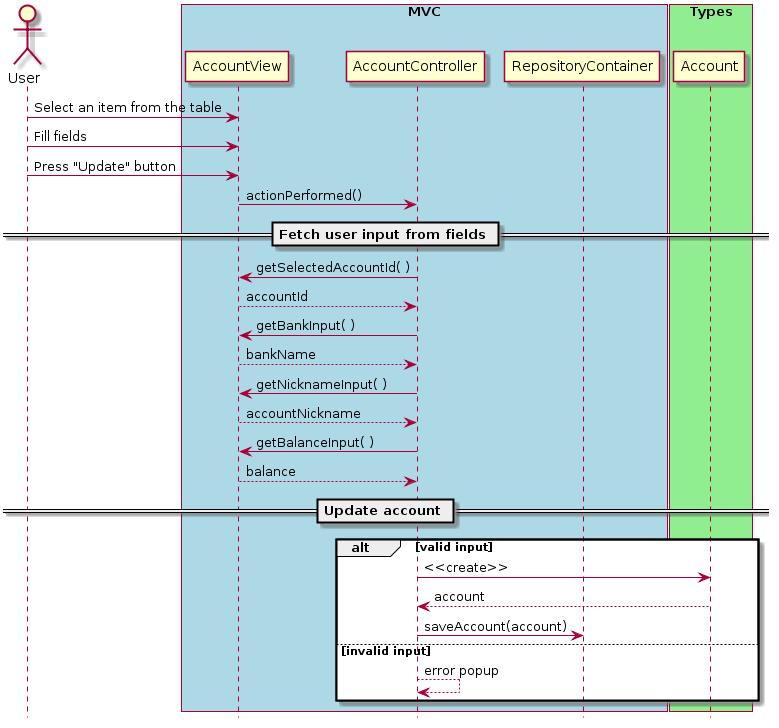
\includegraphics[width=\textwidth,height=\textheight,keepaspectratio]{diagrams/sequence/updateAccount.png}
\captionof{figure}{Updating an account}
\bigskip

\subsection{Delete an account}
To delete an account, the user selects an entry in the \code{AccountView}'s table and clicks the "Delete" button. This sends an \code{ActionEvent} to the \code{AccountController}. The registered listener for this event then calls the \code{deleteAccount()} on the model. \code{Transaction} deletion is handled similarly.\\
\\
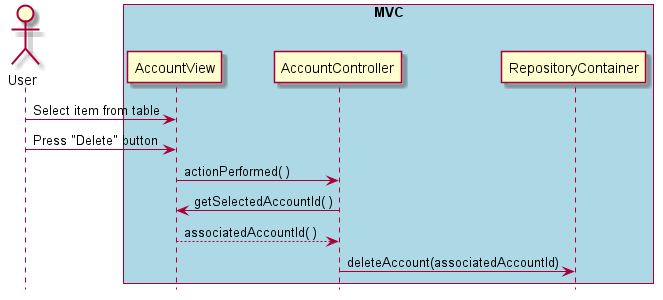
\includegraphics[width=\textwidth,height=\textheight,keepaspectratio]{diagrams/sequence/deleteAccount.png}
\captionof{figure}{Deleting an account}
\bigskip

\subsection{Import a transaction list}
In this scenario, the users imports a list of transactions from a .csv file and adds them to the model. When the user clicks the "Import" button, the \code{TransactionController} creates a window with a dialog box. The user then inputs the file path of the transaction csv file. If the file path is valid, both the file path and the currently selected accountId is passed to the model with a call to \code{importTransactions()}. For details on how the model then handles the import, see \ref{sec:modelImportDetail}.\\
\\
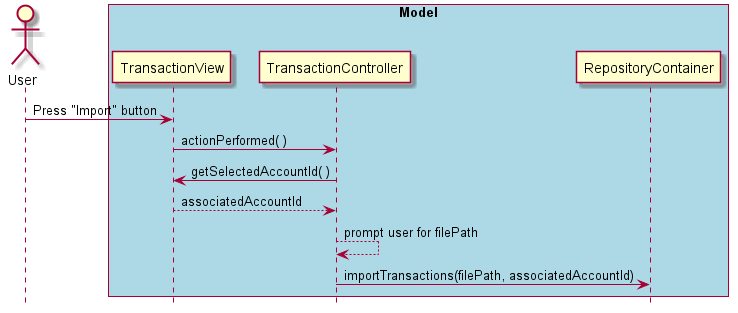
\includegraphics[width=\textwidth,height=\textheight,keepaspectratio]{diagrams/sequence/importHighLevel.png}
\captionof{figure}{Import a list of transactions from .csv file}
\bigskip

\subsection{Model implementation details}
The next subsections offer a glimpse into the internal logic of the model and how it implements the methods of its interface.

\subsubsection{saveAccount()} \label{sec:modelSaveDetail}
The \code{saveAccount(Account)} method provides a simple interface for adding new \code{Account} objects or updating existing ones. When the specified \code{Account} object's \code{accountId} member variable is 0, it is assumed that this is a new entry. Otherwise, the call is treated as an update. \\ 

After the \code{saveItem()} method is called, the \code{AccountRepository} creates an \code{SQLValueMap} object (linked HashMap with keys and values of type String) to store the column-value mapping. \\

If the account is new, then the repository uses the \code{SQLStringFactory} class to build a \code{String} insert query using the (key, value) pairs in the \code{SQLValueMap}. It executes the query by calling \code{updateSQL} from the Database class. The repository then updates the account's ID using the accountId value returned from updateSQL and proceeds to add the new account to the repository's \code{AccountMap}.\\

If the account already exists, then the repository will construct a \code{SQLValueMap} for the where clause of the query using the account's ID. \code{SQLStringFactory} is then used to generate an update query, which will be executed by calling the \code{Database} class's \code{updateSQL} method. The returned accountId is unused. \\
\\
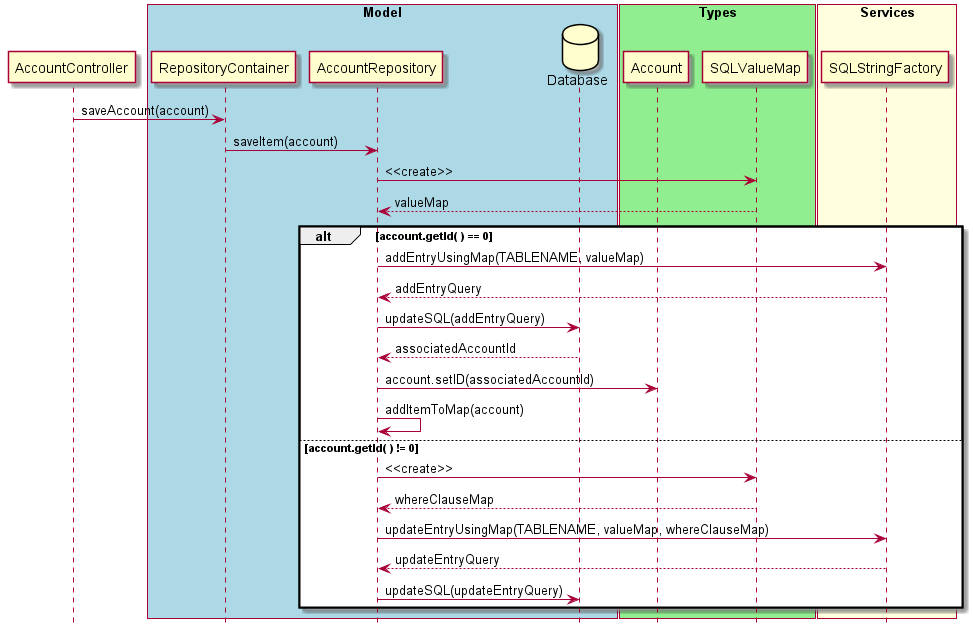
\includegraphics[width=\textwidth,height=\textheight,keepaspectratio]{diagrams/sequence/addAccountImp.png}
\captionof{figure}{Model - Saving an account}
\bigskip

\newpage
\subsubsection{importTransactions()} \label{sec:modelImportDetail}
The \code{importTransaction()} method first creates a \code{BufferedReader} using the file path. Then, it iterates over the file, line by line, using the \code{BufferedReader}'s \code{readLine()} method. \\

The line is split into tokens using the \code{split()} method. Using the returned array of tokens, a \code{Transaction} object is constructed. The model then saves the new\code{Transaction} object by calling its own \code{saveTransaction()} method.\\
\\
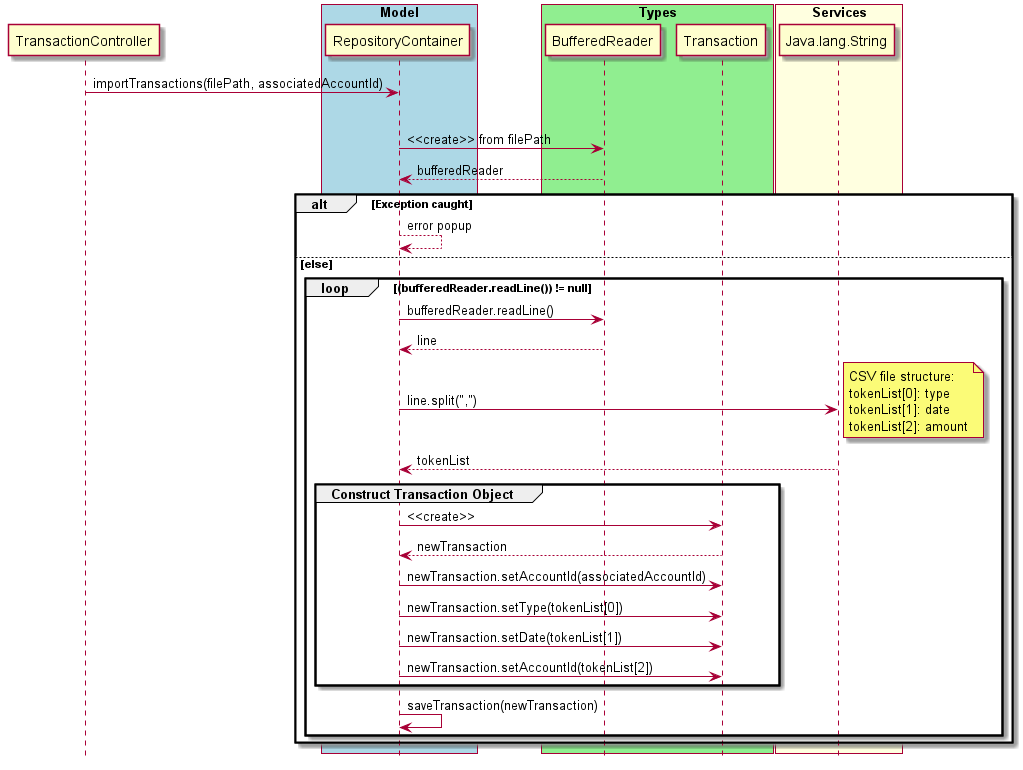
\includegraphics[width=\textwidth,height=\textheight,keepaspectratio]{diagrams/sequence/importLowLevel.png}
\captionof{figure}{Model - Import list of transactions from .csv file}
\bigskip


\end{document}
